\section{Drift Chamber Calibration Procedures}
In this section, we discuss the calibration procedures used to obtain the 
best possible spatial resolution for reconstructing the trajectory of
a forward-going charged particle.  We need to know three things to 
accurately reconstruct a trajectory: the location of the wires, the
distance of closest approach (DOCA) of the track to the wire and the
value of the magnetic field traversed.  These were determined by
\begin{itemize}
\item alignment procedures
\item time to distance calibration
\item magnetic field mapping and modelling
\end{itemize}.  


\subsection{Alignment Procedures}
\label{align}

\hskip 0.15in
Each of the 18 drift chambers was 
surveyed with millimeter to sub-millimeter
accuracy, but we wanted an independent check of the chambers' positions and 
we needed to know the absolute position to about 0.1 mm in order to 
achieve momentum resolutions on the order of 0.3\%.  For 
these reasons, the survey values for the chamber geometry were viewed only as 
a reasonable starting point to be refined by comparisons with data.

To adjust the chamber geometry parameters to improve the tracking resolution,
``straight-track'' data, with the torus magnetic field off, were analyzed.  
Tracks were found and fitted with our standard track reconstruction package.
For various bins in the angle of the track, we measured the shifts of the
track residual means as a function of layer number. 
Before correcting for mis-alignment in software, the data showed significant 
displacements of the means from zero, as large as 2 mm.  

Our alignment procedure considered only the relative alignment of the
three drift chambers in any particular sector to each other.
Our only inter-sector constraint was that all sectors, after alignment,
should point to a common target vertex.

Our procedure was straight-forward.  On a first pass through
the data we used misaligment parameters (shifts and rotations of individual
chambers) set to zero.  On subsequent passes, we deliberately misaligned
a particular chamber by a particular offset in position or angle and 
produced a second set of plots of residual mean vs. layer.  We ran 18 passes
through the data, adjusting all combinations of region (1, 2, 3) and
of offset type $\delta$x, $\delta$y, $\delta$z, $\theta$x, 
$\theta$y, $\theta$z, one at
a time.  The offsets in $x, y$ and $z$ were 2 mm, and the angular rotations
were 0.2 degrees.  These 2mm shifts and 0.2 degree rotations were
called ``unit distortions''.

We then subtracted the pass1 residual distribution from a pass``i'' distribution
to give a ``change of residual'' distribution caused by a given ``unit distortion''.
We then fit the observed residual distribution from the data to a weighted
sum of the 18 ``change of residual'' distributions.  In principle, we
could have had 18 free parameters, but in practice we had 12 free parameters:
 $\delta$ x, $\delta$ y, $\delta$ z, and $\theta$ y for each of the 3 chambers: R1, R2 and R3,
where $\theta y$ is a tilt of a chamber.  The yaw ($\theta x$) and roll ($\theta z$)
were not varied because they did not improve the fits.

Fig.~\ref{resids-vs-layer-before} plots the mean of the residuals of a straight-line
fit to the tracks versus layer (1 - 36 layers of the chambers), for each sector.
The misalignment is plainly visible as a noticeable shift of the residual means
from zero.  The bulk of the offsets occurs in shifts of groups of 12 layers which
corresponds to one physical chamber (a R1 chamber has layers 1-12, R2 from 13-24 and
R3 from 25-36).  

%%%%%%%%%%%%%%%%%%%%%%%%%%%%%%%%%%%%%%%%%%%%%%%%%%%%%%%%%%%%%%%%%%%%%%%%%%%
\begin{figure}[htbp]
\vspace{10cm}
\begin{picture}(50,50)
\put(-10,10)
{\hbox{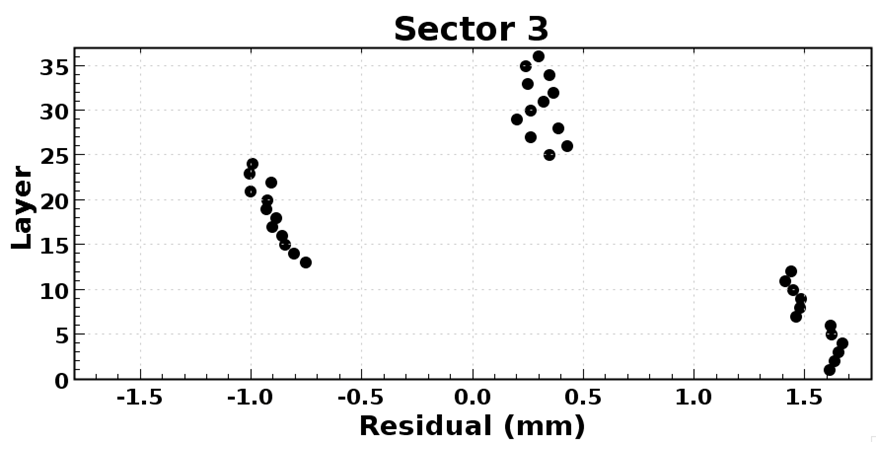
\includegraphics[width=1.\textwidth,natwidth=610,natheight=642]{img/resids-vs-layer-before.png}}}
\end{picture}
\caption{\small{A plot of the fit residual mean versus layer, before alignment.}}
\label{resids-vs-layer-before}
\end{figure}
%%%%%%%%%%%%%%%%%%%%%%%%%%%%%%%%%%%%%%%%%%%%%%%%%%%%%%%%%%%%%%%%%%%%%%%%%%%

Because our ``unit distortions'' are not orthogonal functions, we needed to do a simultaneous
fit over four angular ranges; because two ``unit distortions'' which are highly correlated in
one angular range were usually not in other ranges.  In addition to minimizing the residuals
from our 36 drift chamber layers, we also include a 37th term in the residual sum: the 
distance of closest approach to the beam target vertex.  As mentioned before this helped
to align the chambers sector to sector.

Figure~\ref{resids-vs-layer-before} is the misalignment before our aligning procedure, while
Fig.~\ref{resids-vs-layer-after} shows the shifts of the means which remain after we have
aligned the chambers.

%%%%%%%%%%%%%%%%%%%%%%%%%%%%%%%%%%%%%%%%%%%%%%%%%%%%%%%%%%%%%%%%%%%%%%%%%%%
\begin{figure}[htbp]
\vspace{10cm}
\begin{picture}(50,50)
\put(-10,10)
{\hbox{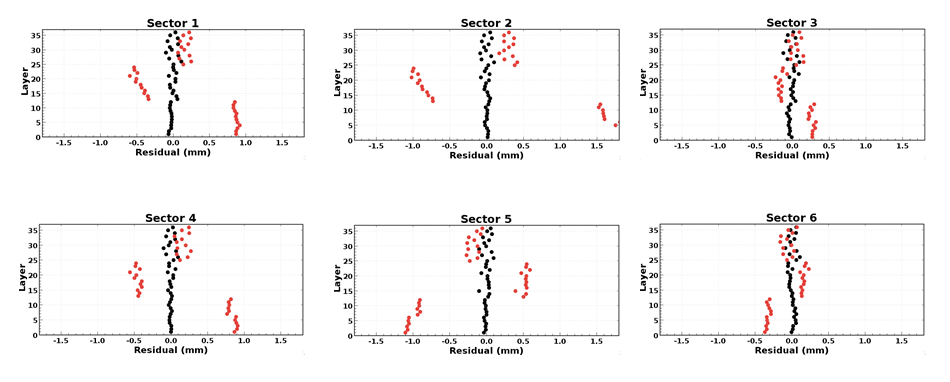
\includegraphics[width=1.\textwidth,natwidth=610,natheight=642]{img/resids-vs-layer-after.png}}}
\end{picture}
\caption{\small{A plot of the fit residual mean versus layer, after alignment.}}
\label{resids-vs-layer-after}
\end{figure}
%%%%%%%%%%%%%%%%%%%%%%%%%%%%%%%%%%%%%%%%%%%%%%%%%%%%%%%%%%%%%%%%%%%%%%%%%%%

The 
results of this procedure indicated that the best-fit position of the chambers 
along the three coordinate axes varied by up to several millimeters relative 
to the surveyed positions.  Our best estimate of the final average offset of 
the chambers after alignment was approximately 65$\mu m$.

\subsubsection{Geometrical Distortions}
The drift chamber internal geometry (placement of wires, etc.) was checked by detailed
surveys of the endplate, and of the endplates position with respect to the survey holes
located on the `nose' and `back' plates during construction of the full chamber assembly
and before stringing.
As discussed in the previous section, we surveyed the chambers into place on the
torus and also applied a `straight-track' analysis to fine-tune our knowledge
of the chambers geometrical location and orientation.

In addition to these alignment procedures which treat the chamber as a rigid, fixed
geometrical shape, we also measured and corrected two important chamber distortions:
\begin{itemize}
\item wire sagging due to gravity
\item bowing inward of the endplates in response to the collective wires' tension
\end{itemize}

The wire sag can be a large as 1mm for our 4 m long wires.  For this small
sag, it is sufficient to describe the shape of the sag as a parabola with
maximum deviation from a straight line occurring at the mid-plane of the chamber.
This correction to the hit position is thus applied at `event time' when 
the y-location of the hit has been determined.

The second type of geometrical distortion is due to the bowing of the endplates.
Because we wished to keep the endplates as thin as possible and because we did
not wish to obstruct the active area of the chamber volume with material, the
entire tension load was borne by the endplates which had a simple support at the
small `nose' plate and a fixed support at the 'back' plate.

We did extensive engineering analysis and also post-stringing survey to determine the
size and pattern of this bowing.  Because our endplate planes are not perpendicular to
the wires, when they bow they move the wire endpoints outward.  The amount varies
according to the chamber position because the weight of the endplates also plays a role,
but the bowing in the direction perpendicular to the wire could be as large as 1.5 mm.
This point of maximum deflection occurs about a fourth of the way between the `nose' and
`back' plates.  In Fig.~\ref{sketch-of-distortions} we show the engineering analysis
for a R2 enplate which agreed well with our direct surveys.

%%%%%%%%%%%%%%%%%%%%%%%%%%%%%%%%%%%%%%%%%%%%%%%%%%%%%%%%%%%%%%%%%%%%%%%%%%%
\begin{figure}[htbp]
\vspace{5cm}
\begin{picture}(50,50)
\put(-10,10)
{\hbox{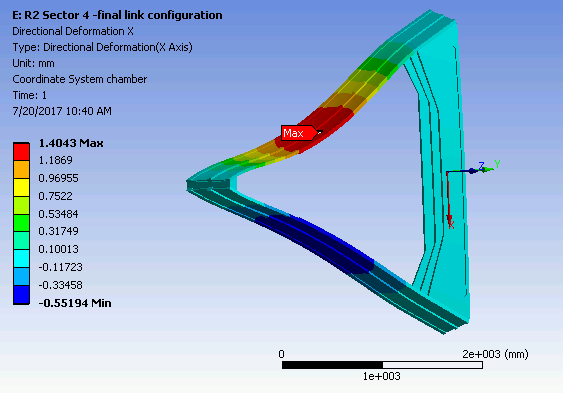
\includegraphics[width=1.\textwidth,natwidth=610,natheight=642]{img/sketch-of-distortions.png}}}
\end{picture}
\caption{\small{An engineering analysis showing the endplate bowing due to wire tension.}}
\label{sketch-of-distortions}
\end{figure}
%%%%%%%%%%%%%%%%%%%%%%%%%%%%%%%%%%%%%%%%%%%%%%%%%%%%%%%%%%%%%%%%%%%%%%%%%%%

\subsection{Time to Distance Calibration}
The drift chamber Time to Digital Converters (TDC) measure time.  
These TDC units are part of our overall Drift Chamber Readout Boards (DCRB) and
have an intrinsic resolution of 1 ns or better; too small to be relevant to
our overall time to distance calibration.

First, the digitized time is corrected for a number
of effects, and this corrected time is converted to a Distance of Closest Approach (DOCA), by 
a pre-calculated time to distance function.  In this subsection we 
explain the time corrections, the function used to calculate time as a 
function of DOCA and how we calibrate the parameters of this function.

\subsubsection{Time Corrections}
The drift time is the elapsed time between the time that the particle 
traversed the wire cell and the time that the released gas ions (electrons)
reached the sense wire.

The drift time is given by the following expression:
\begin{equation} 
\label{drift}
t_{drift} = t_{tdc} - t_{start} - t_{0} - t_{flight} - t_{prop} - t_{walk},
\end{equation}

\noindent
where $t_{tdc}$ is the raw time measured by the TDC, $t_{start}$ is the event start time, 
$t_0$ is the fixed-time (cable) delay for the wire, $t_{flight}$ is the 
flight time of the particle from the interaction vertex to the wire, $t_{prop}$ 
is the signal propagation time along the wire, and $t_{walk}$ is a time-walk 
correction made for short drift times due to different ionizations for slow 
and fast particles.  
With a trigger based on detecting an electron in the CLAS12 detector, the event start time is 
given by the time-of-flight counter time for the primary scattered electron 
corrected for the calculated flight time of this electron from the beam-target vertex.

As indicated in equation~\ref{drift}), the fixed-time delays (mainly fixed cable delays) 
for each wire must be known in order to determine the drift times.   To determine
this t$_0$ value, we produced a histogram of the following quantity for all hits
used on tracks:$ ( t_{tdc} - t_{start} - t_{flight} - t_{prop} - t_{walk} )$.
This produced a characteristic plot of a drift chamber signal on a flat
background from out-of-time tracks.  Our 24,192 drift chamber signals are carried
on individually made multi-conductor cables which each carred 16 signals.  We thus
produced and analysed 24,192/16 = 1512 histograms to determine that many values of
t$_0$. We occasionally re-do this analysis whenever we have a new trigger condition
or new configuration of readout boards.


\subsubsection{Time-to-Distance Functional Parameterization}
\label{tdistcal}

\hskip 0.15in
Each hit on a track is characterized by two variables, the measured drift 
time from the sense wire and the Distance of Closest Approach to the 
sense wire resulting from the track fit. 
Note, we refer to variants of DOCA: one is ``TRKDOCA'' which is the
fit value of the track's closest approach to the wire and ``DOCA''
which is the best estimate of this distance, as calculated from the time.
 
A best fit to the dependence of DOCA on time defines the 
drift-velocity function of the drift cells. However, several factors 
complicate this analysis. For example, the DOCAs obtained from the fitted 
tracks are biased quantities since an initial estimate of the drift-velocity 
function is used in the track determination.  Moreover, the drift cells are 
not circular, as the analysis implicitly assumes, but are hexagonal, leading 
to angle-dependent corrections.   Also, the R2 chambers are in a 
region of high and spatially varying magnetic field.  Finally, the different 
ionization densities of the tracks from particles with different velocities 
leads to substantial time-walk corrections for tracks near the wire.  Each of 
these points is briefly discussed in this section.

Fig.~\ref{garfield-isochrones} shows the isochrone contours and electric-field lines for 
a representative R3 and R2 cell.  Note that the contours are circular close 
to the wire but become hexagonal near the outer boundaries of the cell.  This 
illustrates the necessity of knowing the entry angle of the track in order to 
determine the drift distance to the sense wire from the measured drift time.

%%%%%%%%%%%%%%%%%%%%%% Figure : Garfield Picture %%%%%%%%%%%%%%%%%%%%%%%%%%
\begin{figure}[htpb]
\vspace{4.5cm} 
\special{psfile=img/garfield.eps hscale=49 vscale=49 hoffset=-15 voffset=-130}
\caption{\small{Plot of electric-field lines and equal-time isochrone contours
(100 ns interval) for a 90$\%$ argon - 10$\%$ CO$_2$ gas mixture for (a) an R3
drift cell where two rays are drawn highlighting two different track entrance 
angles of $\alpha$ = 0$^{\circ}$ and 30$^{\circ}$, and (b) an R2 cell that 
was assumed to be located within a uniform 1~T magnetic field along the z 
direction.}}
\label{garfield-isochrones}
\end{figure}
%%%%%%%%%%%%%%%%%%%%%%%%%%%%%%%%%%%%%%%%%%%%%%%%%%%%%%%%%%%%%%%%%%%%%%%%%%%

\subsubsection{Function Parameterization}
\label{funcpar} 

In the CLAS detector, the drift distance was parameterized and fit as a function
of drift time.~\cite{mdm95}
For CLAS12, we have instead chosen to parameterize the time as a function of
distance.  This is a more natural description of the drift chamber signal
for several reasons:
\begin{itemize}
\item the maximum drift distance is given by geometry (the distance from
a sense wire to the nearest field wire) and so it is fixed
\item the drift velocity is a function of electric field strength, so the
point of minimum field is the point of minimum velocity (and thus the inflection point on the T vs X curve). 
This inflection point of the curve occurs at a
definite value of distance within the cell and not at a definite value of time.
\item the time walk due to finite ionization is
naturally parameterized as a function of distance and not as a function of time.
\item two of the major time corrections (time walk which is a function of the
particle $\beta$ and a time correction for wires in a magnetic field, $B$ which
scales like $B^2$) can simply be added to the nominal functional form.
\end{itemize}

A {\bf single functional form} is used to fill two tables: one of time indexed by discrete
values of distance for use in the simulation by GEMC and one of 
distance indexed by time for use by the track reconstruction code.


\subsubsection{Choice of Mathematical Form for the Distance to Time Function}
We use a 4th order polynomial to model the distance to time relationship.

\begin{equation}
t(x) =  a x^4 + b x^3 + c x^2 + d x,
\end{equation}


By the use of simple calculus we convert the parameters a, b, c and d to equivalent parameters which have
a physically intuitive meaning.

\subsubsection{Physical Constraints on the Drift Velocity Function}

Inspection of  Fig.~\ref{garfield}a reveals that for tracks near the outer
edge of the cell, the first arriving ions follow the electric-field line from 
the field wire to the sense wire, independent of track entrance angle.  The
corresponding drift time is referred to as $t_{max}$ and occurs when DOCA is at its maximum value,
called ``Dmax''.

A second constraint is that the velocity near the wire is the ``saturated drift
velocity'' for our gas mixture, 90$\%$ argon - 10$\%$ CO$_2$.  We call this parameter $V_0$.

A third constraint is imposed by the fact that there is a definite point in the
cell at which the electric field is a minimum.  This implies that this is the point
of minimum velocity and is thus an inflection point.  This occurs at a value
$r = (x/Dmax) /approx 0.64$ and the drift velocity at this point is termed $V_{mid}$.

A summary of constraints on the function coefficients:
\begin{itemize}
\item  $t(x)$ must equal $t_{max}$ when $x = Dmax $.
\item  the drift velocity near the sense wire ($x = 0$)
must equal the saturated value, $V_0$
\item the function has an inflection point (a
mininum in velocity) at the point in the cell with the lowest electric field
strength.  From the geometry of our cells, this occurs at a distance
of $\approx 0.64 \times Dmax$.  Finally,
\item the velocity equals $V_{mid}$ at the inflection point.
\end{itemize}

These are the equations defining the constraints:
\begin{enumerate}
\item $t(x = Dmax) = t_{max}$
\item $dt / dx (x = 0) = 1 / V_0$
\item $d^2 t / dx^2 (\hat{x} = 0.64 ) = 0$   
\item $dt / dx (\hat{x} = 0.64 ) = 1/V_{mid}$  
\end{enumerate}

In this way we convert our original parameters, a, b, c and d to the physically meaningful
parameters $t_{max}, V_0, r, and V_{mid}$ where $r$ is the value 0.64 (the fractional distance
at which the inflection point occurs) which can in principle also be varied.


\subsubsection{Dependence of Distance to Time Function on Local Angle}
\noindent
The preceding was the derivation for the function of time as a function
of drift distance for tracks with a local angle, $\alpha = 30^0$.  
We now discuss the
functional dependence on varying local angle and on non-zero and varying
values of the B-field.

Please refer back to Fig.~\ref{garfield} which shows a 0 degree track and a 30 degree
track, both at maximum distance from the sense wire.  Note that they will produce
a signal hit with the same time, Tmax, even though their distance-of-closest-approach d
iffers by a factor
of $cos(30^{0})$.  If Dmax is the distance from sense to field wire (and the maximum
DOCA possible for a 30 deg. track), then Dmax times $\cos(30^\circ-\alpha)$ is the maximum
DOCA for a track with local angle, $\alpha$.  Call this distance, $Dmax_{\alpha}$.

\subsubsection{Local Angle Dependence of Polynomial Form}
We derived the function for time versus distance for a particular local angle, $\alpha$, by
assuming the same functional form as for $\alpha = 30$ but with a {\bf different coefficient, a}, which 
satisfies the constraint that  $F(dmax_{\alpha},\alpha)$ = $t_{max}$.

Using this constraint, we can solve for $a_{\alpha}$ in terms of the known coefficients $V_0, ~a, ~n$, and $m$,
yielding the following:
\begin{equation}
\label{aalphaequation}
a_{\alpha} = {{t_{max} - b ~dmax_{\alpha}^3 - c ~dmax_{\alpha}^2 - d ~dmax_{\alpha}}\over{dmax_{\alpha}^4}}
\end{equation}

Using this formula for $a_{\alpha}$ we can derive the time as a function of distance and local
angle, $\alpha$ as shown in Fig.~\ref{xvst}.  See, for instance, the upper-left sub-figure 
which shows the time as function of distance for 5 different angles between $0^{\circ}$ and 
$30^{\circ}$, equally spaced in $\cos \left(30^\circ-\alpha\right)$.  Note two things:
\begin{enumerate}
\item for each angle, $\alpha$, the time is $t_{max}$ at $dmax_{\alpha}$, and
\item the distances for a given time vary with angle, $\alpha$, as $\cos \left(30^\circ-\alpha\right)$.
\end{enumerate}

The general functional form for time as a function of distance and local angle, $\alpha$
is given by
\begin{equation}
\label{tfunctionofxandlocalangle}
t(x,\alpha) = a_{\alpha} x^4 + b x^3 + c x^2 + d x
\end{equation}

\subsubsection{Dependence of Distance to Time Function on Magnetic Field Strength}
Since the R2 chambers are located within the field region of the CLAS torus, the 
magnetic field affects the drift velocity as shown in 
Fig.~\ref{xvst}b.  In particular, the field rotates and shrinks the isochrones
as shown in Fig.~\ref{garfield}b.  These effects can be modeled by a 
modification to the effective entrance angle of the track and by an increase 
in the time at a particular DOCA.  Both of these corrections are assumed to depend only on the 
magnitude of the magnetic field, and not its direction, following a study 
described in Ref~\cite{MM-IEEE}.  

The rotation of the isochrones is parameterized as a shift in the effective
entrance angle.  
\begin{equation} 
\label{eq-bcorrn-to-ang}
\alpha_b = \alpha_0 + \alpha_c \cos^{-1}(1 - a B), 
\end{equation}

The correction term $\alpha_c$ is determined from a 
GARFIELD simulation to be:

\begin{equation} 
\label{eq-bang}
\alpha_c = \cos^{-1}(1 - a B), 
\end{equation}

\noindent
where $a$ is a constant equal to $0.02$ and $B$ is the magnetic field strength in Tesla and angular
units are degrees.

%%%%%%%%% Figure : TRKDOCA vs. Drift Time -- Angle and Field Dependence %%%%%%%%%%
\begin{figure}[htb]
\vspace{15.cm} 
\special{psfile=img/tvsx.eps hscale=80 vscale=80 hoffset=-20 voffset=-10}
\caption{\small{Scatterplot of the corrected drift time versus TRKDOCA for 
(upper-left) R1, showing curves for various local angles from 30$^{\circ}$
(righmost curve) to 0$^{\circ}$ (leftmost curve).  (Upper-right) for R2; 
additionally showing 3 bands for B-field magnitudes of 0, 1, 1.5 Tesla.
(Lower-left) for R3 with the inflection point identified.}}
\label{xvst}
\end{figure}
%%%%%%%%%%%%%%%%%%%%%%%%%%%%%%%%%%%%%%%%%%%%%%%%%%%%%%%%%%%%%%%%%%%%%%%%%%%%%%%


The maximum drift time used in the time-to-distance function was extracted 
directly from the data.  For R2 the maximum drift time was parameterized as:

\begin{equation} 
\label{eq-bmax}
t_{max}(B) = t_{max}(0) + b B^2,
\end{equation}

\noindent
where $b$ is a constant and $B$ is the magnetic field strength.

At any given local magnetic field point, the distance-to-time function 
includes an additional correction term $\delta t_B$ to describe 
the magnetic field dependence.  See this reference~\cite{qin96} for a related
parameterization of the change in the distance at a particular time due to a
B-field. 

\begin{equation}
\label{XTB}
t(\hat{x},\alpha,B) = t(\hat{x},\alpha-\alpha_c, B=0) +  \beta(\hat{x})*B^2.
\end{equation}

\noindent
In this expression, the first term is the time calculated assuming B=0, and the
second term is the time increase due to the B field.  For the R1 and R3 functions, no magnetic field 
dependence is included, as the chambers are located outside the torus 
cryostats in regions that are relatively field-free.

\section{Determining the Distance to Time Function Parameters}
Each hit on a track is characterized by two parameters, the measured drift 
time from the sense wire and the distance-of-closest-approach (TRKDOCA) to the 
sense wire.  A best fit to the dependence of time on TRKDOCA determines the
values of the parameters of the drift-velocity function. 
We determine the optimized values of these function parameters by fitting
a histogram of $TRKDOCA$ vs. time, data-basing the fit paramters, re-doing
the track fitting, and iterating.

To illustrate our fits, in Fig.~\ref{calcdoca-and-trkdoca-vs-time} we show a plot of
the data (time vs TRKDOCA) and overplotted is the function (time vs. CALCDOCA).
The function does a fair job of following the shape of the data.

%%%%%%%%% Figure : calcdoca and trkdoca plotted vs time %%%%%%%%%%
\begin{figure}[htbp]
\vspace{5cm}
\begin{picture}(50,50)
\put(-10,10)
{\hbox{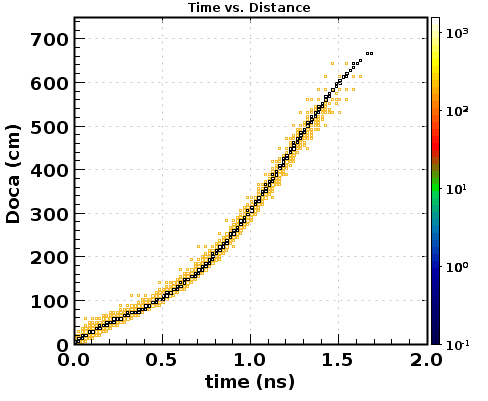
\includegraphics[width=1.\textwidth,natwidth=610,natheight=642]{img/calcdoca-and-trkdoca-vs-time.png}}}
\end{picture}
\caption{\small{A plot of TRKDOCA vs. time from our track fits; overplotted in darker symbols
is the calculated distance (CALCDOCA) vs. time.}}
\label{calcdoca-and-trkdoca-vs-time}
\end{figure}
%%%%%%%%%%%%%%%%%%%%%%%%%%%%%%%%%%%%%%%%%%%%%%%%%%%%%%%%%%%%%%%%%%%%%%%%%%%%%%%

\section{Using the Distance to Time Function in Reconstruction}
The track reconstruction program needs to know the expected distance as a function
of time.  However, as explained in the previous paragraph, we will have calibrated and fitted
the observed time as a function of distance.  So, we need to NUMERICALLY INVERT the t=f(x)
function in order to fill a table of X (real number) as a function of the time index (integer).

\subsubsection{Filling the Time to Distance and Distance to Time Tables}
We calibrate the distance to time function by fitting the drift time versus
TRKDOCA at a particular local angle, $\alpha$.  We write the independent parameters,
$V_0, ~V_{mid}$ and $T_{max}$ to the data-base.  At the beginning of a reconstruction program,
an {\bf inversion program} is run to numerical invert the function to produce a table
of distance indexed by time.


\subsubsection{How to Interpolate and Extrapolate in Local Angle}
Please refer back to Fig.~\ref{xvst} in order to understand the local-angle dependence
of distance versus time.  When the time is equal to $t_{max}$ the distance is equal to
the largest value for the local angle; that is, $dmax_{\alpha}$.  Also note that by
simple geometrical reasoning, $dmax_{\alpha} = dmax$  $cos(30-\alpha)$.
We assume that at times less than tmax and distances less than dmax, the calculated
distances still vary linearly as $cos(30-\alpha)$.  This angle dependence is built into
our functional form.

This means that we
\begin{itemize}
\item {\bf Fill} our time to distance tables for different local angles using the function, and
\item {\bf Interpolate} between time to distance tables for different local angles to obtain
the calculated distance at a particular local angle
\end{itemize}
For example if ``$X_0$'' is the distance (at a particular time) for a table filled for tracks with local angle of 0 degrees
and ``$X_{30}$'' is the corresponding quantity for a table of 30 degree tracks, then
\begin{equation} 
\label{eq-extrap30}
X(t,\alpha) = X_0 + (X_{30}-X_0) (cos(30-\alpha) - cos(30)) / (1. - cos(30))
\end{equation}

\subsection{Magnetic Field Model: A Comparison to Measurement}
In the Fall of 2016, we mapped the magnetic field of the torus magnet.
We documented the equipment and measurements in an article on the
construction of the torus (see Ref.~\cite{torus-ieee}) and in internal
documents (see Ref.~\cite{magmapping}).

We used three independent 1-dimensional Hall probes mounted in a precision-machined
Teflon holder.  The holder was a cylindrical solid which was pushed down a precision
Carbon fiber tube.  The probes were precisely spaced to be 5cm apart in the z-dimension,
with one oriented perpendicular to the z-axis, another perpendicular to the y-axis and
the third perpendicular to the x-axis.  In this way, we measured the x, y and z components
of the magnetic field at z-points separated by 5 cm along the axis of the toroid.

The Carbon fiber tube was positioned in x and y by precision machined ``endplates'' at the
upstream and downstream ends of the torus.  There were 24 precise hole locations on each
plate  (4 between each pair of torus coils).  We measured $B_x, ~B_y, ~B_z$ at 40 
locations in z at each of the 24 x, y locations, resulting in 2880 measurements.

By adjusting the six coils' shapes and locations, we were able to match our
magnetic model to the measurements to an accuracy of $0.5\%$.  Details of this
analysis will be available in a future publication, but in summary we
show in Fig.~$\ref{bmodel-bmeasured}$ the fractional difference between
the magnetic field from our model to that measured for the $40 X 6 = 240$ measurements
taken at 30 cm radius.  This is the region of the highest magnetic field (approx. 2 T)
and is most important for our low-angle, high-momentum tracks.  At the time of publication,
the average fractional difference was about 0.5\%.

%%%%%%%%%%%%%%%%%%%%%%%%%%%%%%%%%%%%%%%%%%%%%%%%%%%%%%%%%%%%%%%%%%%%%%%%%%%
\begin{figure}[htbp]
\vspace{5cm}
\begin{picture}(50,50)
\put(-10,10)
{\hbox{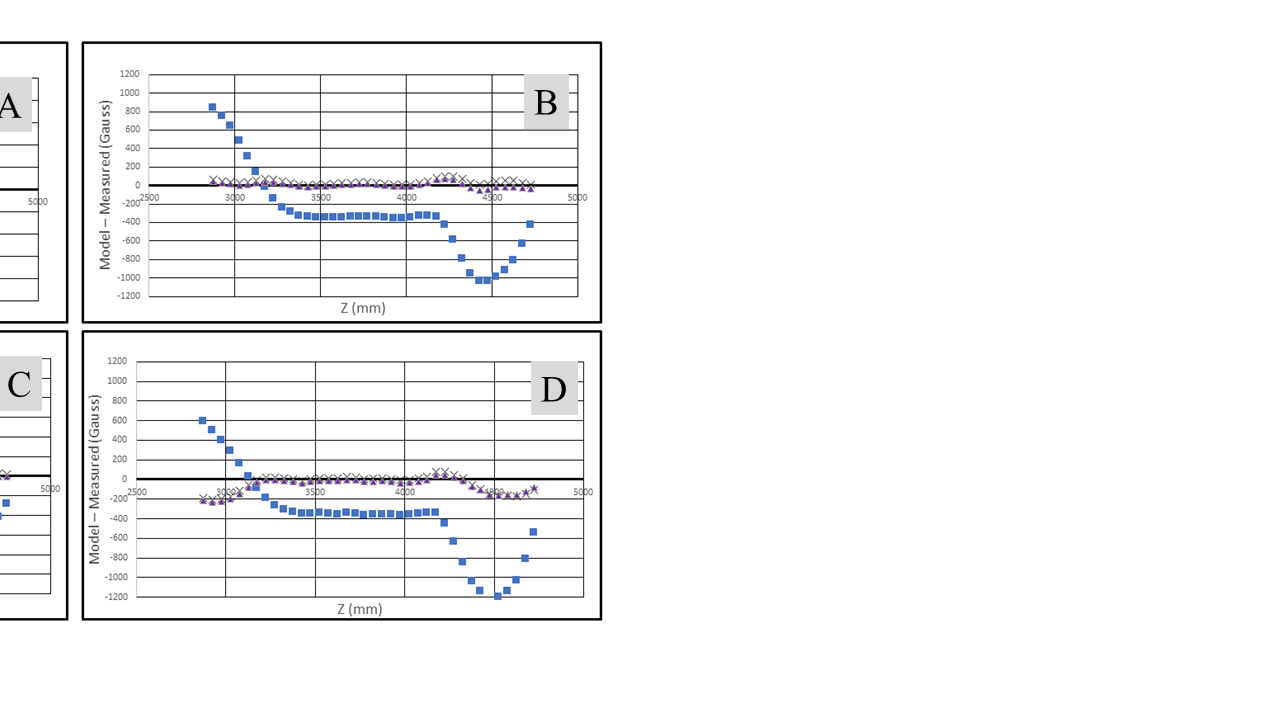
\includegraphics[width=1.\textwidth,natwidth=610,natheight=642]{img/bmodel-bmeasured.png}}}
\end{picture}
\caption{\small{A plot of (Bmodel - Bmeasured) / Bmodel versus z for the 240 measurement points
located at a radius of 30 cm and at the midplane between the 6 torus coils.}}
\label{bmodel-bmeasured}
\end{figure}
%%%%%%%%%%%%%%%%%%%%%%%%%%%%%%%%%%%%%%%%%%%%%%%%%%%%%%%%%%%%%%%%%%%%%%%%%%%

